\section{Introduction}

A low-pass FIR (\textit{Finite Impulse Response}) filter is a type of digital filter used in signal processing to attenuate or remove high-frequency components from a signal, allowing only low-frequency components to pass through. FIR filters are characterized by their impulse response, which is a finite duration sequence of coefficients.
The basic operation of a low-pass FIR filter involves convolving the input signal with the impulse response of the filter. The filter coefficients determine the filter's frequency response, and specifically in a low-pass filter, they emphasize the passage of low-frequency signals and suppress higher frequencies
The design of a low-pass FIR filter involves determining the appropriate filter order (length) and selecting the filter coefficients. The filter order determines the length of the filter's impulse response and affects the sharpness of the filter's frequency cutoff. Higher filter orders generally result in steeper roll-off characteristics but require more computational resources.

% For this project, my main point of interest is exploring the architecture of an FIR filter with the following characteristics:
For this project, I will be focused in exploring the architecture of an FIR filter with the following characteristics:

\begin{itemize}
    \item Sampling frequency: 46 kHz
    \item Pass frequency: 8 kHz
    \item Stop frequency: 9.6 kHz
    \item Number of coefficients:
    \begin{itemize}
        \item Minimum coefficients possible
        \item 20 coefficients
        \item 30 coefficients
    \end{itemize}
    \item Arithmetic:
    \begin{itemize}
        \item Single precision floating point
        \item Fixed point 24 bits
        \item Fixed point 16 bits
        \item Fixed point 8 bits
    \end{itemize}
    \item Optimizations:
    \begin{itemize}
        \item 1 stage multiplier pipelining
        \item 2 stage multiplier pipelining
        \item Multiplier-less using CSD
        \item Distributed Arithmetic
    \end{itemize}
\end{itemize}

The implemented filter has a magnitude response as figure~\ref{fig:fir_mag_response} shows.

\begin{figure}
    \centering
    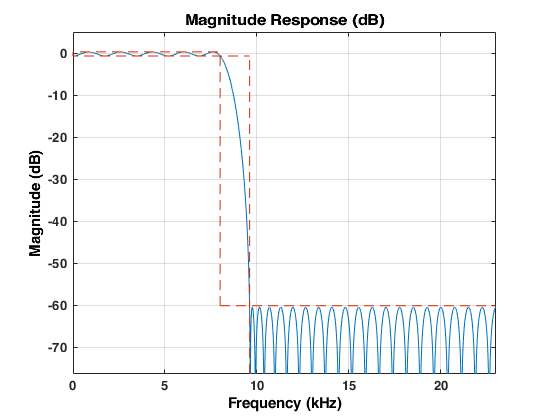
\includegraphics[width=0.4\textwidth]{Images/fir_minimum_mag_response.png}
    \caption{FIR magnitude response}
    \label{fig:fir_mag_response}
\end{figure}